%************************************************
\chapter{Design}\label{ch:design} % $\mathbb{ZNR}$
%************************************************
As stated in the introduction (\autoref{ch:introduction}), the research question is the following: ``How can the cost and waste monitoring of a Cloud Computing application be offered in a scalable and resilient manner?''. In order to investigate the characteristics of the solution for monitoring a Cloud Computing application, it is important to determine the requirements before. The requirements are divided into architectural requirements and waste requirements. The architectural requirements will lead to the proposed architecture, while the waste requirements will lead to a specified algorithm.

\section{Architectural requirements} \label{sec:architectural_req}
As this research is the successor of the work: `Visualizing Computational Waste in Cloud Computing' by A. Spina \cite{spina}, there is some similarity with his architectural requirements. However, his architecture is based on a solution for which a probe collects data from monitored instances, and an aggregator that represents this data into a human-readable format. His relevant requirements are:
\begin{itemize}
    \item The solution should be functional across command cloud providers.
    \item The data should be considered sensitive and secured accordingly.
    \item The solutions should be configurable, but easy to use.
    \item The solution should strike a balance between efficiency and effectiveness.
    \item The solution should collect utilization statistics on the monitored system. 
\end{itemize}

\noindent
In \cite{aceto2013cloud} a number of properties are mentioned. These apply to a distributed monitoring system, and are therefore applicable to the desired solution. The most important properties are:
\begin{itemize}
    \item Scalability: a monitoring system is scalable if it can cope with a large number of probes.
    \item Elasticity: a monitoring system is elastic if it can cope with dynamic changes of monitored entities, so that virtual resources created and destroyed by expansion and contraction are monitored correctly.
    \item Adaptability: a monitoring system is adaptable if it can adapt to varying computational and network loads in order not to be invasive.
    \item Timeliness: a monitoring solution is timely if detected events are available on time for their intended use.
    \item Autonomicity: an autonomic monitoring solution is able to self-manage its distributed resources by automatically reacting to unpredictable changes.
    \item Accuracy: a monitoring system is accurate when the measures it provides are accurate, i.e. they are as close as possible to the real value to be measured.
\end{itemize}

\noindent
Both lists in this section are considered relevant, and the desired solution should be able to meet all these properties. For the implemented solution, the decision has been made to monitor only Docker containers, as this provides a way of abstracting a certain deployment. Therefore, the underlying operating system is not that important. This ensures that the solution will be functional across all OS's that are capable of running Docker containers. 

\section{Architecture} \label{sec:architecture}
As mentioned in \autoref{sec:related_technologies}, the proposed architecture uses state-of-the-art open-source technologies. Several design patterns have been evaluated, such as a Client-Server network and a peer-to-peer network. the latter is considered more scalable, as the number of resources grow with the number of nodes. Additionally, a peer-to-peer system does not have a single point of failure. Therefore, this system is desired over a client-server network. However, as the data is stored in a Prometheus database, and this cannot operate in a peer-to-peer system, another solution is needed. Using the federation technique of Prometheus \cite{prometheus_federation}, the decision has been made to go for a hierarchical network. This proposed network consists of only one root, a number of supernodes, and optional a number of nodes.\\

\noindent
An architectural overview of the three node types, as well as the technologies that are included, can be found in \autoref{fig:architecture}. The only difference between a node and a super node is the Prometheus database. Furthermore, the root is only used to visualize the collected metric data in the Grafana dashboard. Each node type is shortly described below.

\begin{figure}
    \centering
    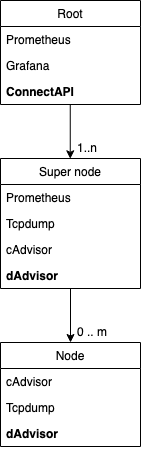
\includegraphics[width=0.3\textwidth]{gfx/architecture.png}
    \caption{Architectural overview}
    \label{fig:architecture}
\end{figure}

\subsection{Root}
The root is a single access point for the displaying the obtained results. Its Prometheus database is dynamically configured, such that it scrapes data from all the super nodes deployed in the system. 
In order to successfully deploy the entire system, the root needs to be deployed first, as it provides an access point for the nodes as well. This access point is implemented in the connect API and further described in ....\todo{add reference}. The connect API distributed the nodes over the available super nodes and ensures that $\floor*{\frac{n}{m}} \leq \frac{n}{m} \leq \ceil*{\frac{n}{m}}$ holds for which $n$ is the number of nodes and $m$ the number of super nodes.

\subsection{Super node}
As explained before, there is only a slight difference between the node and the super node, as the latter deploys Prometheus. This database is automatically configured, such that is scrapes from a set of nodes. The metrics that a super node collects are the same as for a node and are therefore described in the following section.

\subsection{Node}
The node consists of three processes. Resource metrics are collected using the cAdvisor process and internet packets are collected using Tcpdump \cite{tcpdump}.


\section{Waste requirements} \label{sec:waste_requirements}
As explained in the previous subsection, the architectural requirements lead to a solution that is capable of monitoring a set of Docker containers in a SOA. However, there are a few restrictions for the resource utilization of these containers. This is mathematically stated as:

\begin{itemize}
    \item $0 < u_i \leq 1$ for $1 \leq i \leq n$: Every container within a host utilizes a value between 0 (exclusive) and 1 (inclusive). The desired solution will also be a running container, but this resource utilization is filtered from the rest of the utilization values, such that the monitoring solution only collects data about the deployed system.
    \item $\sum_{i=1}^n u_i \leq 1$: The total utilization of a certain set of containers for a given host cannot utilize more than 100\%. And with the previous requirement, its lower-bound is 0 (exclusive). As the total waste is computed as $1 - \sum_{i=1}^n u_i$, it can be concluded that the waste is bounded by 0 (inclusive) and 1 (exclusive).
\end{itemize}

\noindent
Although the mathematical constraints are very trivial, it is important to state this beforehand. Using these utilization requirements, several approaches of computing the resource waste can be assessed. Also, stating these constraints are important as it affects the desired solution.

 